\documentclass{article}
\usepackage{fullpage}
\usepackage[utf8]{inputenc}
\usepackage{pict2e}
\usepackage{amsmath}
\usepackage{enumitem}
\usepackage{eurosym}
\usepackage{mathtools}
\usepackage{amssymb, amsfonts, latexsym, cancel}
\setlength{\parskip}{0.3cm}
\usepackage{graphicx}
\usepackage{fontenc}
\usepackage{slashbox}
\usepackage{setspace}
\usepackage{gensymb}
\usepackage{accents}
\usepackage{adjustbox}
\setstretch{1.35}
\usepackage{bold-extra}
\usepackage[document]{ragged2e}
\usepackage{subcaption}
\usepackage{tcolorbox}
\usepackage{xcolor, colortbl}
\usepackage{wrapfig}
\usepackage{empheq}
\usepackage{array}
\usepackage{parskip}
\usepackage{arydshln}
\graphicspath{ {images/} }
\renewcommand*\contentsname{\color{black}Índice} 
\usepackage{array, multirow, multicol}
\definecolor{lightblue}{HTML}{007AFF}
\usepackage{color}
\usepackage{etoolbox}
\usepackage{listings}
\usepackage{mdframed}
\setlength{\parindent}{0pt}
\usepackage{underscore}
\usepackage{hyperref}
\usepackage{tikz}
\usepackage{tikz-cd}
\usetikzlibrary{shapes, positioning, patterns}
\usepackage{tikz-qtree}
\usepackage{biblatex}
\usepackage{pdfpages}
\usepackage{pgfplots}
\usepackage{pgfkeys}
\addbibresource{biblatex-examples.bib}
\usepackage[a4paper, left=1cm, right=1cm, top=1cm,
bottom=1.5cm]{geometry}
\usepackage{titlesec}
\usepackage{titletoc}
\usepackage{tikz-3dplot}
\usepackage{kbordermatrix}
\usetikzlibrary{decorations.pathreplacing}
\newcommand{\Ej}{\textcolor{lightblue}{\underline{Ejemplo}}}
\setlength{\fboxrule}{1.5pt}
\usepackage{subcaption}
\newcommand{\bboxed}[1]{\fcolorbox{lightblue}{lightblue!10}{$#1$}}
\newcommand{\rboxed}[1]{\fcolorbox{red}{red!10}{$#1$}}

\DeclareMathOperator{\N}{\mathbb{N}}
\DeclareMathOperator{\Z}{\mathbb{Z}}
\DeclareMathOperator{\R}{\mathbb{R}}
\DeclareMathOperator{\Q}{\mathbb{Q}}
\DeclareMathOperator{\K}{\mathbb{K}}
\DeclareMathOperator{\im}{\imath}
\DeclareMathOperator{\jm}{\jmath}
\DeclareMathOperator{\col}{\mathrm{Col}}
\DeclareMathOperator{\fil}{\mathrm{Fil}}
\DeclareMathOperator{\rg}{\mathrm{rg}}
\DeclareMathOperator{\nuc}{\mathrm{nuc}}
\DeclareMathOperator{\dimf}{\mathrm{dimFil}}
\DeclareMathOperator{\dimc}{\mathrm{dimCol}}
\DeclareMathOperator{\dimn}{\mathrm{dimnuc}}
\DeclareMathOperator{\dimr}{\mathrm{dimrg}}
\DeclareMathOperator{\dom}{\mathrm{Dom}}
\DeclareMathOperator{\infi}{\int_{-\infty}^{+\infty}}
\newcommand{\dint}[2]{\int_{#1}^{#2}}

\newcommand{\bu}[1]{\textcolor{lightblue}{\underline{#1}}}
\newcommand{\lb}[1]{\textcolor{lightblue}{#1}}
\newcommand{\db}[1]{\textcolor{blue}{#1}}
\newcommand{\rc}[1]{\textcolor{red}{#1}}

\renewcommand{\CancelColor}{\color{lightblue}}

\newcommand{\dx}{\:\mathrm{d}x}
\newcommand{\dt}{\:\mathrm{d}t}
\newcommand{\dy}{\:\mathrm{d}y}
\newcommand{\dz}{\:\mathrm{d}z}
\newcommand{\dth}{\:\mathrm{d}\theta}
\newcommand{\dr}{\:\mathrm{d}\rho}
\newcommand{\du}{\:\mathrm{d}u}
\newcommand{\dv}{\:\mathrm{d}v}
\newcommand{\tozero}[1]{\cancelto{0}{#1}}
\newcommand{\lbb}[2]{\textcolor{lightblue}{\underbracket[1pt]{\textcolor{black}{#1}}_{#2}}}
\newcommand{\dbb}[2]{\textcolor{blue}{\underbracket[1pt]{\textcolor{black}{#1}}_{#2}}}
\newcommand{\rub}[2]{\textcolor{red}{\underbracket[1pt]{\textcolor{black}{#1}}_{#2}}}

\usepackage{matlab-prettifier}

\lstset{
	language=Matlab,
	basicstyle=\ttfamily,
	keywordstyle=\color{blue},
	commentstyle=\color{green!70!black},
	stringstyle=\color{red},
	showstringspaces=false,
	breaklines=true,
	numbers=left,
	numberstyle=\tiny,
	stepnumber=1,
	numbersep=5pt,
	frame=single,
	backgroundcolor=\color{lightgray!10},
	captionpos=b,
	tabsize=2,
	inputencoding=utf8,
	literate={á}{{\'a}}1 {é}{{\'e}}1 {í}{{\'i}}1 {ó}{{\'o}}1 {ú}{{\'u}}1{ñ}{{\~n}}1{Ñ}{{\~N}}1{€}{{\texteuro}}1
}

\title{Práctica 1 de Señales y Sistemas\\
Generación de señales discretas y transformaciones de 
la variable independiente}
\author{Francisco Javier Mercader Martínez\\ Rubén Gil Martínez}
\date{}

\begin{document}
\maketitle
\section{Generalización de señales discretas}
\begin{itemize}[label=$-$]
	\item Genere la señal $x[n]$
	
	\begin{lstlisting}
x = [0 0 -0.4 -0.74 -0.2 0 0.5 0.8 1.2 0.8 0.4 0 -0.3 0 0];
	\end{lstlisting}
	\item Genere el eje temporal
	
	\begin{lstlisting}
N = floor(length(x)/2);
n = [-N:N];
	\end{lstlisting}
	\item Dibuje la señal $x[n]$
	
	\begin{lstlisting}
stem(n,x,'.')
	\end{lstlisting}
	\item Muestre el valor de la señal para el instante $n=-3$
\begin{lstlisting}
x(find(n==-3))
\end{lstlisting}
\begin{figure}[h]
	\centering
	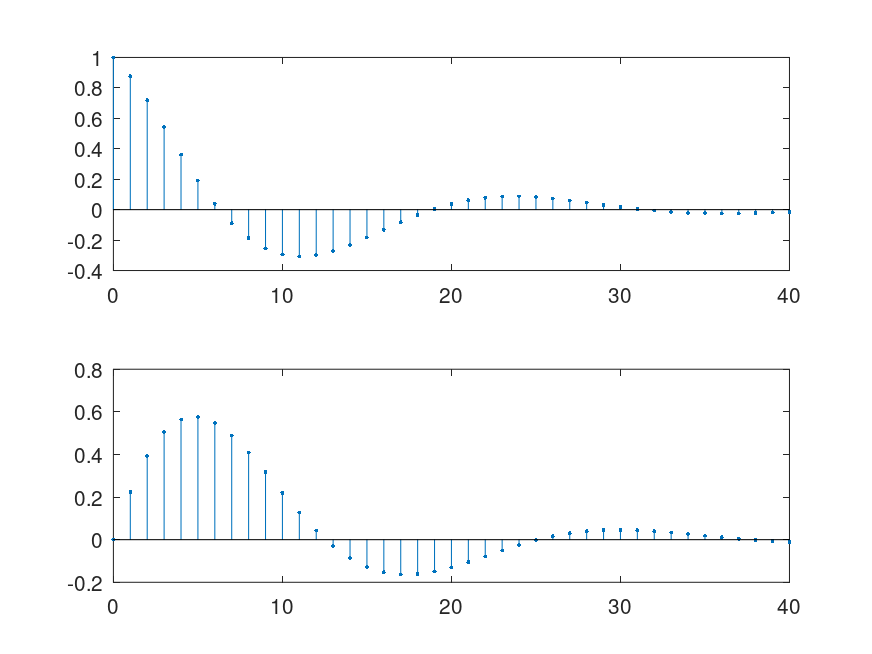
\includegraphics[width=\linewidth]{Imagénes/figure1}
\end{figure}
	\item Modifique el valor de la señal, $x[-3]=-0.6$
\begin{lstlisting}
x(find(n==-3))=-0.6;
\end{lstlisting}
\end{itemize}
\textbf{Cuestiones:}

Utilizando las variables creadas en el ejercicio anterior:
\begin{itemize}[label=$-$]
	\item Genere la señal $y[n]=(-1,1)^n$
	

	\item Genere la señal $x2[n]=y[n]\cdot x[n]$
	\item Genere $z[n]=0.75\cdot(x[n]+x2[n])$
	\item Genere la señal $E[n]=x[n]\cdot x[n]$ o $E[n]=x^2[n]$
	\item Calcule la energía y la potencia de $x[n]$
\end{itemize}

\pagebreak

\begin{lstlisting}
% Cuestiones ejercicio 1:
% Generación de señales:
y = (-1.1) .^ n
x2 = x .* y
z = 0.75 .* (x + x2)
E = x .^ 2

% Energía y potencia de de la señal x:

energia = sum(x .^ 2)
potencia = (1 / (2 * N + 1)) * sum(x .^ 2)
\end{lstlisting}
\begin{verbatim}
y =
-0.51316 0.56447 -0.62092 0.68301 -0.75131 0.82645 -0.90909 1 -1.1 1.21 -1.331 1.4641 -1.6105 1.7716 -1.9487
x2 =
-0 0 0.24837 -0.51226 0.45079 0 -0.45455 0.8 -1.32 0.968 -0.5324 0 0.48315 0 -0
z =
0 0 -0.11372 -0.9467 -0.11191 0 0.034091 1.2 -0.09 1.326 -0.0993 0 0.13736 0 0
E =
0 0 0.16 0.5625 0.36 0 0.25 0.64 1.44 0.64 0.16 0 0.09 0 0
energia = 4.302500
potencia = 0.286833
\end{verbatim}
\section{Transformaciones en la variable independiente}
\subsection{Desplazamiento temporal}

Cree el fichero \textbf{\textit{desplazamiento.m}} con el editor de MATLAB: \textbf{\texttt{File -> New -> m-file}}. Copie el código anterior y guárdelo.

\begin{lstlisting}
% Archivo "desplazamiento.m"
funtion y=desplazamiento(x,n0)
long=length(x);               % longitud de x
if(n0 >= 0)                 % Si n0 es =>0
	y=[zeros(1,n0) x(1:long-n0)];       % desplazamiento a la derecha
else                     % si n0 es <0
	n0=-n0;
	y=[x(1+n0:long) zeros(1,n0)];       % desplazamiento a la izquierda
end
\end{lstlisting}
\begin{itemize}[label=$-$]
	\item Compruebe el correcto funcionamiento de dicha función ejecutando las siguientes instrucciones:
	
	\begin{lstlisting}
% Cuestiones ejercicio 2: Desplazamiento temporal

x = rand(1,15);
n = -7:7;
y = desplazamiento(x,1);
subplot(2,1,1)
stem(n,x,'.')
subplot(2,1,2)
stem(n,y,'.')
	\end{lstlisting}
	\item Ejecute retardos 2 (2 muestras hacia la derecha) y $-3$ (3 muestras hacia la izquierda) y represente las gráficas correspondientes comprobando el correcto funcionamiento de la función.
	
	\begin{lstlisting}
y1 = desplazamiento(x,2);
figure(3)
stem(n,y1,'.')

y2 = desplazamiento(x,-3);
figure(4)
stem(n,y2,'.')
	\end{lstlisting}
\end{itemize}


\begin{center}
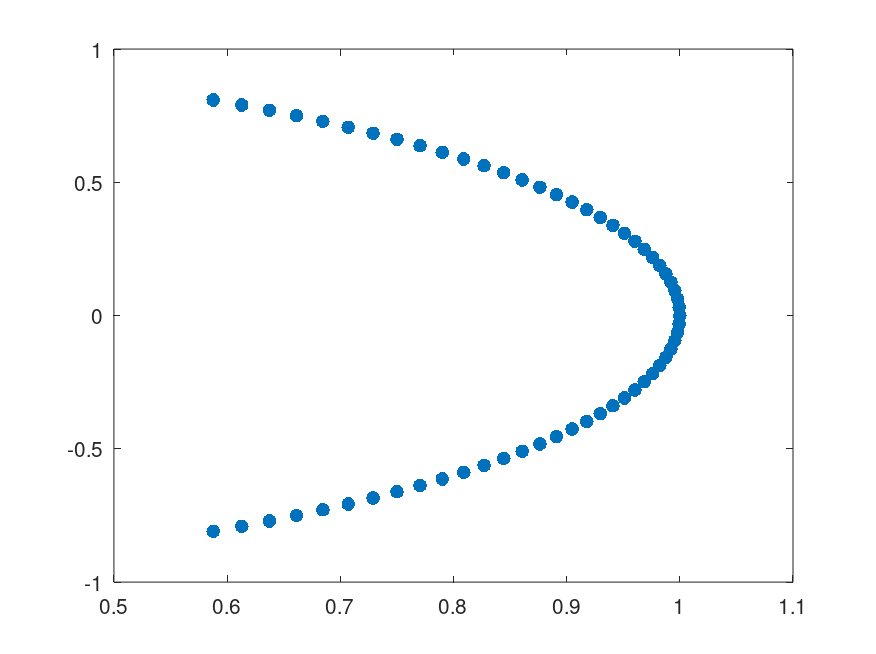
\includegraphics[width=0.45\linewidth]{Imagénes/figure3}
\qquad
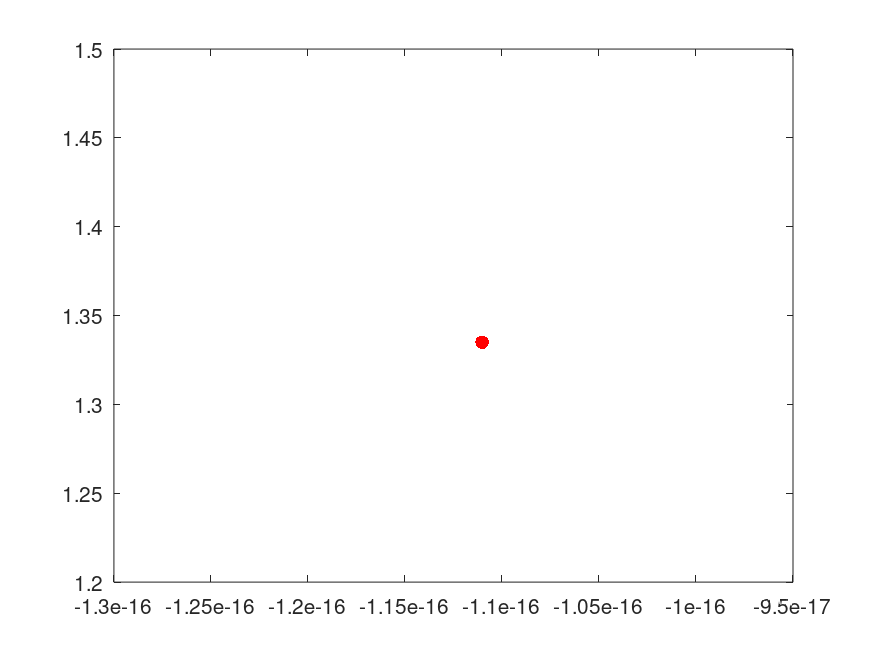
\includegraphics[width=0.45\linewidth]{Imagénes/figure4}
\end{center}
\subsection{Inversión temporal}
\begin{itemize}
	\item Apartado 1
	\begin{lstlisting}
		x1=[1 1 2 3 5 8 13 21 34];
		n = 0:8;
		
		y1 = inversion(x1,n);
		figure(5)
		subplot(2,1,1)
		stem(n,x1,'.', "LineWidth", 1.5)
		subplot(2,1,2)
		stem(n,y1,'.', "LineWidth", 1.5)
		
		x2=[1 -2 3 -4 5 -4 3 -2 1]
		n = -4:4;
		
		y2 =inversion(x1,n);
		figure(6)
		subplot(2,1,1)
		stem(n,x2,'.', "LineWidth", 1.5)
		subplot(2,1,2)
		stem(n,y2,'.', "LineWidth", 1.5)
	\end{lstlisting}
	
	\begin{center}
			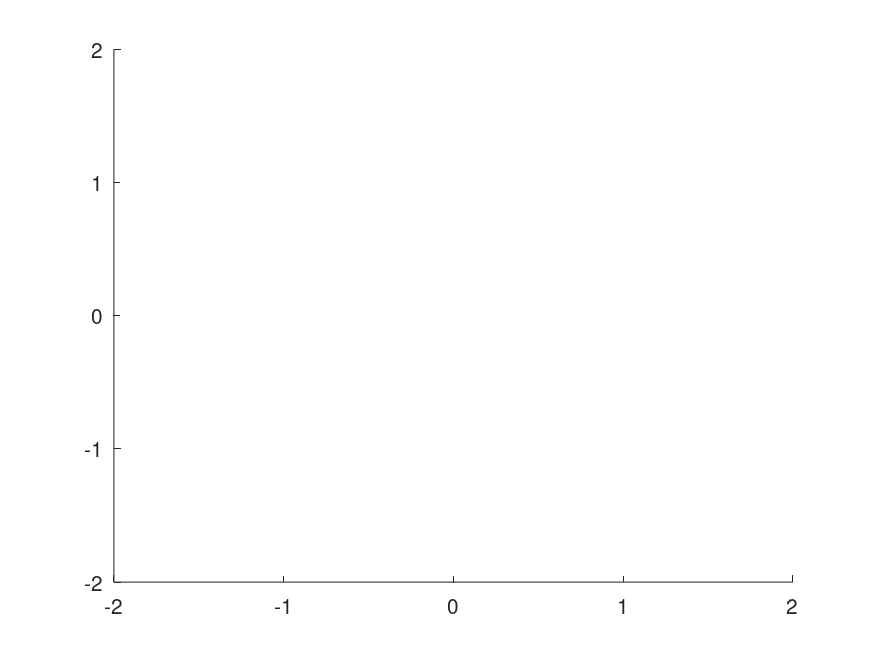
\includegraphics[width=0.45\linewidth]{Imagénes/figure5}
		\qquad
		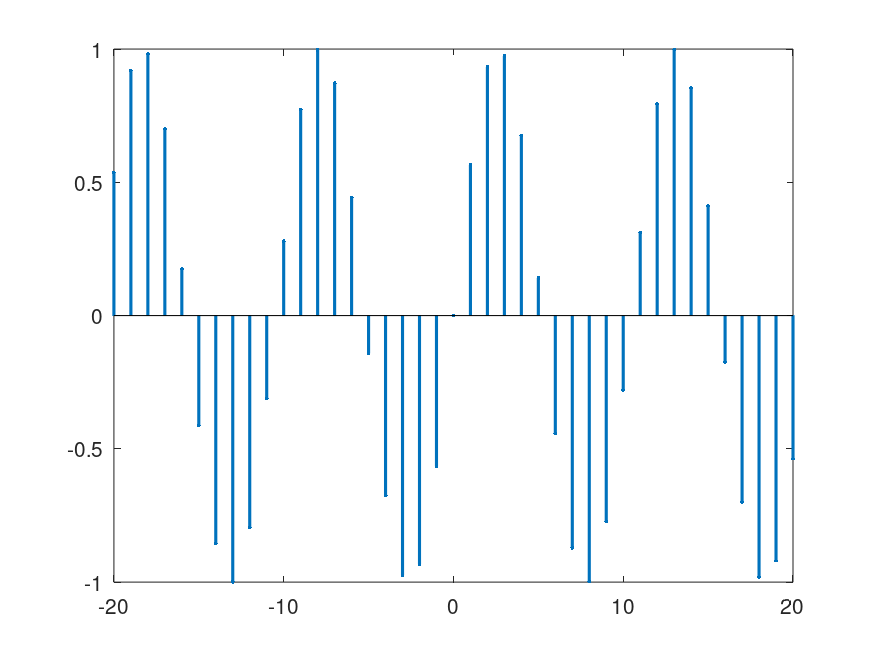
\includegraphics[width=0.45\linewidth]{Imagénes/figure6}
	\end{center}
	\item Apartado 2
	
	Lo que ocurre con \texttt{y2} es que se invierte pero podemos apreciar que no es simétrica, al contrario que \texttt{y1}, que si lo es.
\end{itemize}
\section{Señales periódicas}
\textbf{Ejercicios:}
\begin{lstlisting}
x=randn(1,9);
x=[x x x x x];
N=floor(length(x)/2);
n=[-N:N];

figure(7)
subplot(2,1,1)
stem(n,x,'.', "LineWidth", 1.5)

n2=[-20:20];
i0=find(n==n2(1));


subplot(2,1,2)
stem(n2,x(i0:i0+length(n2)-1), "LineWidth", 1.5)
\end{lstlisting}
\begin{center}
	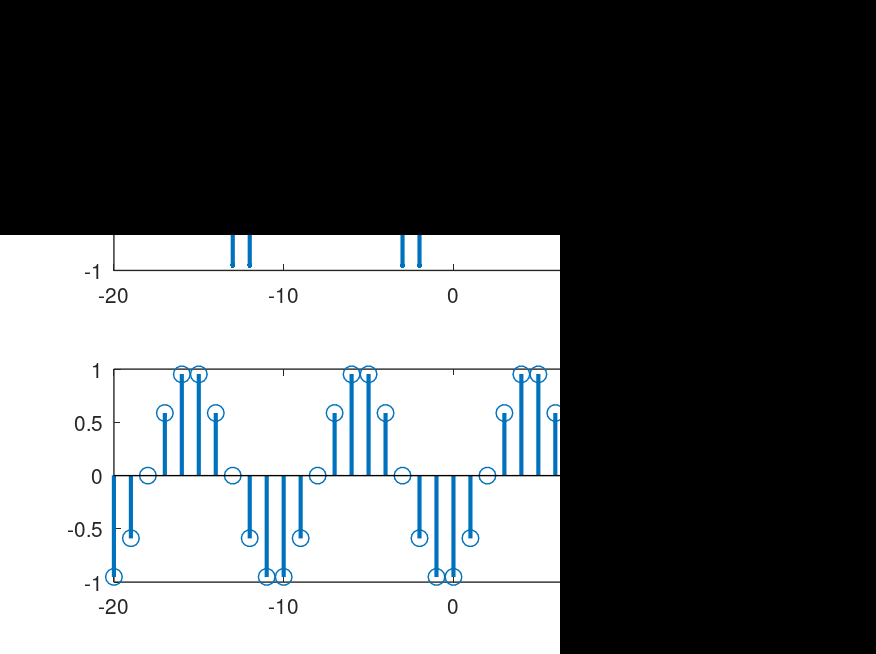
\includegraphics[width=\linewidth]{Imagénes/figure7}
\end{center}
\textbf{Cuestiones:}
\begin{lstlisting}
n=[-100:100];
x = sin(pi / 5 * n)
N_x = (2*pi) / (pi/5)
% N_x = 10

n=[-20:20];
x = sin(pi / 5 * n)

y = sin(pi / 5 * (n - N))
figure(8)
subplot(2,1,1)
stem(n,x,'.', "LineWidth", 1.5)

subplot(2,1,2)
stem(n,y, "LineWidth", 1.5)
\end{lstlisting}
\begin{center}
	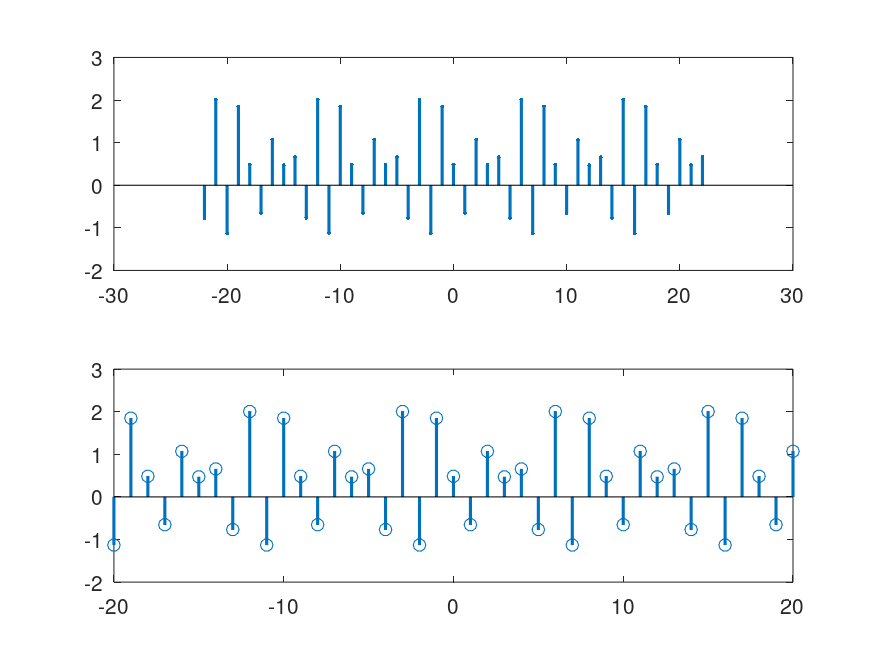
\includegraphics[width=\linewidth]{Imagénes/figure8}
\end{center}
\begin{lstlisting}
n = [-100:100];
y = sin(0.6 .* n);

n = [-20:20];
y = sin(0.6 .* n);

figure(9)
stem(n,y,'.', "LineWidth", 1.5)
\end{lstlisting}
\begin{center}
	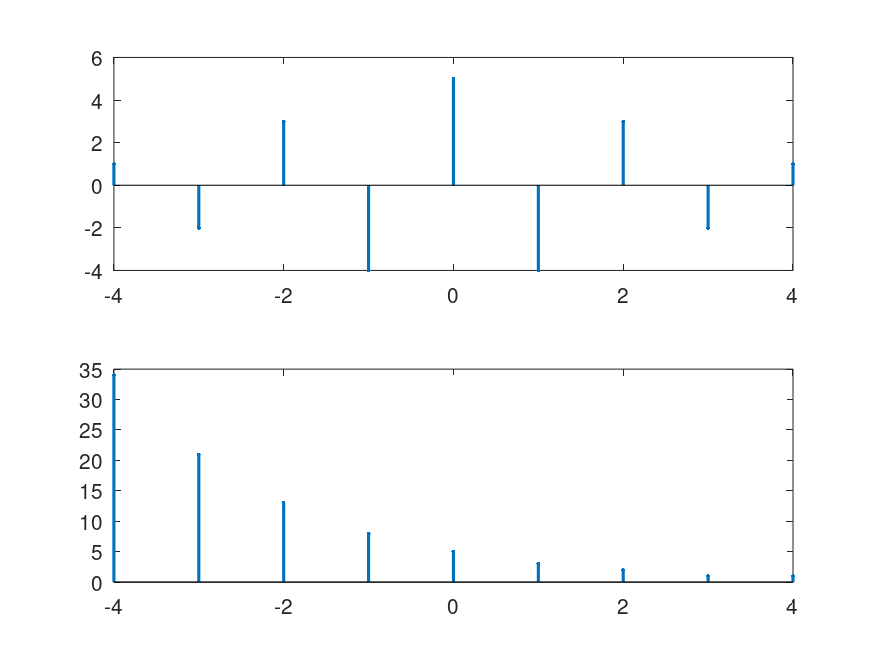
\includegraphics[width=\linewidth]{Imagénes/figure9}
\end{center}
Es similar porque se trata de una función seno, que es periódica pero al multiplicarse por 0.6 se produce una expansión, como se puede apreciar en la gráfica

\begin{lstlisting}
n = [-20:20];

N=floor(length(y)/2);

y2 = desplazamiento(y, -N)
z = y - y2

figure(10)
stem(n,z,'.', "LineWidth", 1.5)
\end{lstlisting}

Se puede ver en la gráfica que z[n] no es periódica
\section{Exponenciales complejas}
\textbf{Ejercicio}

\begin{lstlisting}
z1 = 1.2 + 0.75*j;
z2 = 0.5 + 0.8*j;

cla reset
axis([-2 2 -2 2])
hold on

figure(11)
plot(z1, 'b.', 'MarkerSize', 20)
plot(z2, 'g.', 'MarkerSize', 20)
plot(z1*z2, 'r.', 'MarkerSize', 20)

abs(z1)
angle(z1)

n = [-30:30];

x = exp(j*0.01*pi*n);

figure(12)
plot(x, '.', 'MarkerSize', 20)

hold off
figure(13)
subplot(2,1,1)
stem(n,real(x),'.')
subplot(2,1,2)
stem(n,imag(x),'.')
\end{lstlisting}

\begin{center}
	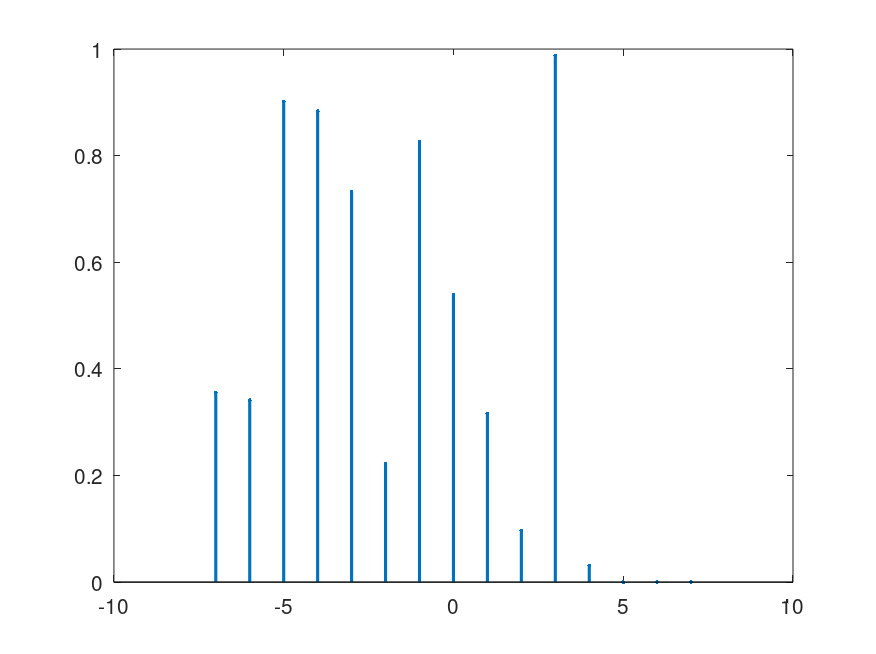
\includegraphics[width=0.5\linewidth]{Imagénes/figure11}
	\qquad
	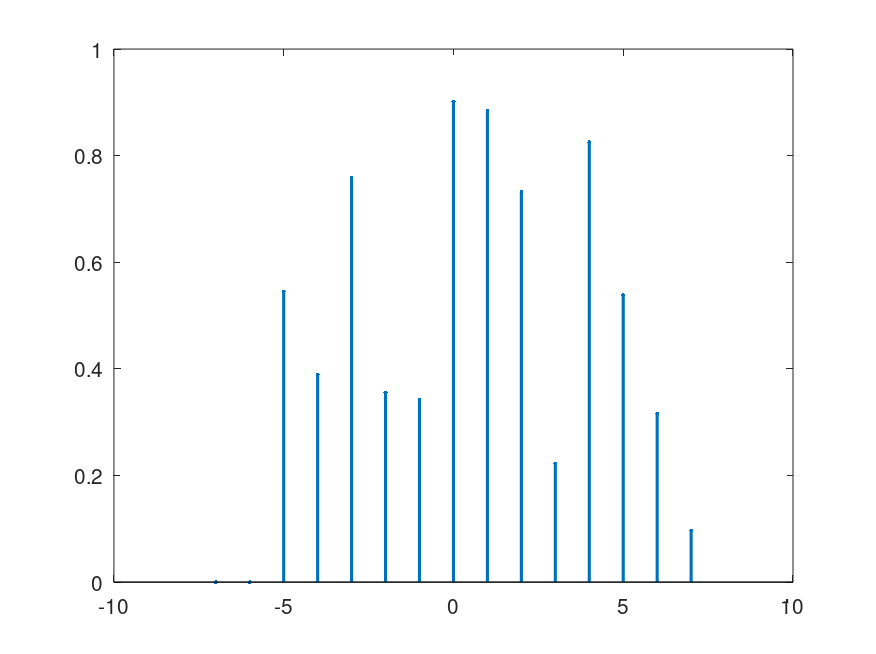
\includegraphics[width=0.5\linewidth]{Imagénes/figure12}
	\qquad
	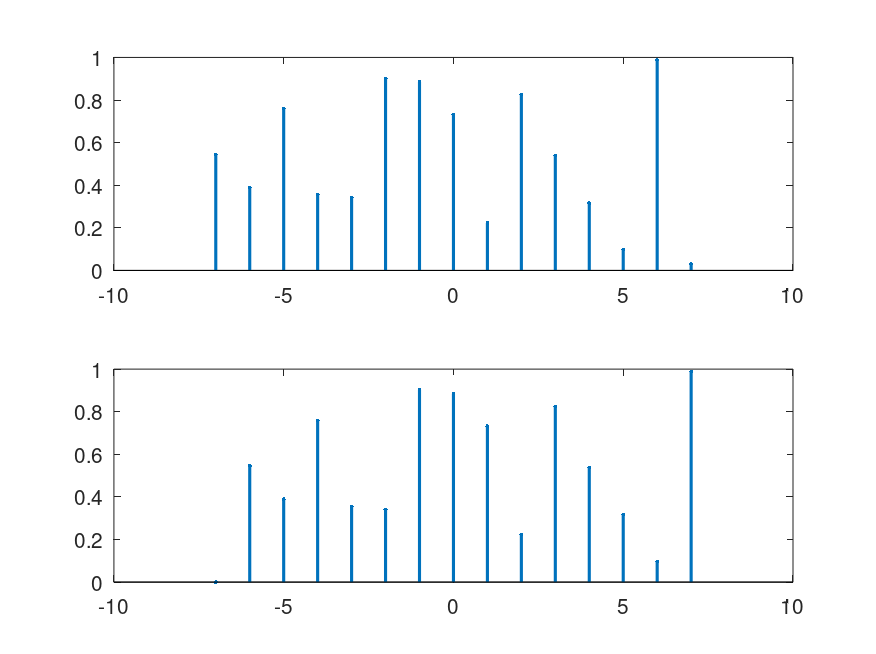
\includegraphics[width=0.5\linewidth]{Imagénes/figure13}
\end{center}
\textbf{Cuestiones:}
\begin{lstlisting}
n = [0:40];
x = exp(-n/10+j*n/4);
figure(14)
subplot(2,1,1)
stem(n,real(x),'.')
subplot(2,1,2)
stem(n,imag(x),'.')

modulo = abs(x);
fase = angle(x);

% modulo = 1.4151
% fase = 0.5586
\end{lstlisting}
\begin{center}
	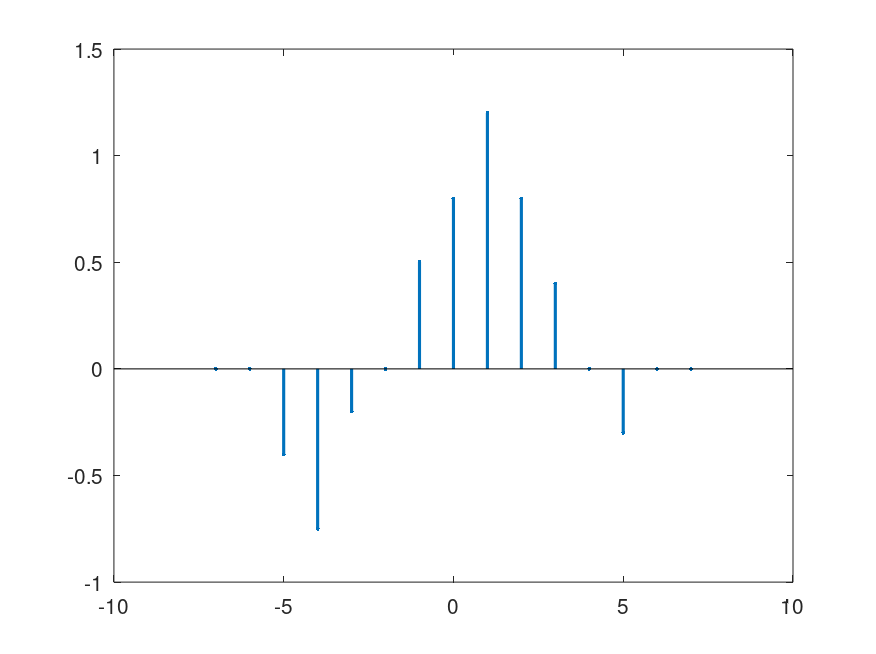
\includegraphics[width=\linewidth]{Imagénes/figure14}
\end{center}
\end{document}